\documentclass[a4paper]{article}
\usepackage{fullpage}
\usepackage{parskip}
\usepackage{titlesec}
\usepackage{xcolor}
\usepackage{url}
% \usepackage[colorlinks = true,
%             linkcolor = blue,
%             urlcolor  = blue,
%             citecolor = blue,
%             anchorcolor = blue]{hyperref}

\usepackage[backend=biber,maxcitenames=1]{biblatex}
\bibliography{library}

\usepackage{graphicx}
\usepackage[space]{grffile}
\usepackage{latexsym}
\usepackage{textcomp}
\usepackage{multirow,booktabs}
\usepackage{amsfonts,amsmath,amssymb}
% You can conditionalize code for latexml or normal latex using this.
\newif\iflatexml\latexmlfalse
\usepackage[utf8]{inputenc}
\usepackage[english]{babel}

\iflatexml
\documentclass[]{article}
\fi
% \usepackage[style=authoryear,backend=biber]{biblatex} % Not (yet) supported by LaTeXML.
\usepackage[]{booktabs}
\usepackage[]{tikz}


% First macro on next line not (yet) supported by LaTeXML: 
% \usetikzlibrary{shapes,arrows,positioning}


\begin{document}

\title{Machine Learning -- Final Report}

\author{Volker Strobel}

\date{\today}

\maketitle

\begin{abstract}
This report presents the techniques and results of a classification
  problem involving missing data as well as a mixture of categorical
  and continuous data. The problem of missing data points is
  addressed by Multiple Imputation Chained Equations. The
  classification is conducted using an ensemble of several classifiers. The
  method was evaluated locally using cross-validation and
  remotely on a hold-out test-set using the Kaggle platform. The best
  Kaggle submission resulted in an accuracy of $85.494\,\%$, which corresponds to
the $3^{\text{rd}}$ position out of $23$ participants in the competition.%
\end{abstract}%
\section{The Challenge}
\label{sec:introduction}

The Kaggle competition ``Final Assignment
IN4320''\footnote{\url{https://inclass.kaggle.com/c/final-assignment-in43202}}
asks participants to predict whether a person earns more than EUR 40k
a year from $D = 13$ predictor variables. The provided dataset was
created by a census bureau. The task can be divided into the following
three challenges:

\begin{itemize}
\item Imputation of missing data points
\item Handling a mixture of categorical and continuous independent variables
\item Classification of the output variable
\end{itemize}

In this report, the terms \emph{wealthy} or ``label 1" describe a sample with income EUR $>40K$ and \emph{non-wealthy} or ``label 0" are used otherwise.

In Section~\ref{sec:analysis}, I analyze and visualize
the structure of the data to set the stage for the classification pipeline. In
Section~\ref{sec:methods}, the used methods for imputation, classification, and transductive learning are detailed. Section~\ref{sec:results} presents and discusses the results obtained during cross-validation and on
Kaggle.

\section{Analysis \& Ideas}
\label{sec:analysis}

To motivate the used classifier, design and technique
choices, I start with an analysis of the given dataset and introduce possible concepts and ideas. Additionally, important patterns dependence structures are visualized.

In total, 13 features are given, of which 8 are categorical and 5 continuous (Table~\ref{tab:features}).
%shows the discrete and continuous features.
The training set consists of 10500 samples and the test set has 38342 samples, resulting in a ratio of approximately $1:3.7$.
The test set is thus considerably larger than the training set.
%and generalization performance is particularly important.
Since transductive learning is permitted, the information in the test set---information about the distribution of the variables---could help to increase the classification performance.

\begin{table}[h]
  \centering
  \begin{tabular}{cc}
    \toprule
  Categorical  & Continuous                     \\
    \midrule
    work class & age                            \\
    education  & number of years of education   \\
marital status & income from investment sources \\
occupation     & losses from investment sources \\
relationship   & working hours per week         \\
race           &                                \\
sex            &                                \\
native country &                                \\
      \bottomrule
  \end{tabular}
  \caption{{Overview of the used features}}
  \label{tab:features}
\end{table}

10500 samples constitute the training set of which 2500 (23\,\%) were labeled as wealthy and 8000 (77\,\%) as non-wealhty. If we assume that the training and test set were randomly sampled from the entire dataset, therefore, the predictions on the test set should reflect this ratio. Additionally always predicting non-wealthy should give a 0-1 loss of 77\,\% under this assumption, which can be used as a baseline for the classifier performance. The assumption can be tested by probing the testset with a ``0-only" submission. This ratio might be useful for setting the class-weights of a classifier or for determining the decision threshold in a decision function: if a classifier is able to output probabilities for the class labels, one would predict ``label 1'', if the probability for ``wealthy'' is greater than the threshold $\theta = 0.5$. However, $\theta$ could be modified, to increase or decrease the amount of ``label 1'' predictions.

In total, approx. $20\,\%$ of the data values are missing, with approx. $23\,\%$ for the variables workclass and occupation, $20\,\%$ for country of origin, and $19\,\%$ for the remaining variables. There is no apparent difference in the percentage and pattern of missing data between the training and the testset. Only $6\,\%$ of samples in the training set and in the test set are complete cases (i.e., have no missing values), making handling missing data a crucial step. I assume that the higher values for the variables workclass, occupation, and country stem from missing values in the original dataset and the missing values for the remaining variables were just introduced. 

Given the description of the dataset and the total number of samples
(48842), the dataset is potentially the UCI Adult Data
set~\cite{lichman2013}. This would underline the pattern of missing
data. A possible method would be to use the labeled samples of the UCI
dataset and match them with the given testset, which should give an
accuracy of 1.0. However, this method is not as straight-forward as it
may seem. The UCI dataset is split in a different manner into training
and testset (amount of training samples: 32561, test samples:
16281). Additionally, the categorical variables in the UCI dataset are
encoded as strings, while in the given dataset, they are encoded as
integers. Therefore, one would have to find a mapping from strings to
integers. The large amount of missing data might impede this
endeavor. Since using the UCI Adult dataset might defeat the goal of
this assignment, I did not take any steps in this direction. A
comparison on
\url{http://www.cs.toronto.edu/~delve/data/adult/adultDetail.html}
shows that the best performing classifier is a Forward Sequential
Selection (FSS) naive Bayes model with an accuracy of $85.95\,\%$. The
classifiers were trained after removing unknown values (7\,\% of
values had missing values; training set size: 30162, test set size:
15060). This accuracy can be used as an indicator of a good
performance on the given dataset. However, there are two differences
to the given dataset: (i) the original UCI dataset had a lower amount
of missing data, and (ii) the UCI dataset had a higher number of
training samples.

\section{Methods}
\label{sec:methods}

\subsection{Missing Data Values}

Missing data values are a common problem in statistics. The failure of
sensors, or the concealment of data impede machine learning
accuracy. Thus, methods have been put forth for the imputation of
missing data points, such as case deletion or single mean
imputation~\cite{schafer2002missing}. However, such simple methods
often discard useful information and are are likely to give a rather
poor result if a large part
of the data is missing.

For using an off-the-self imputation technique the data should ideally
be Missing Completely At Random (MCAR)---there is no dependence
structure between the missing data and any values. Little's MCAR
test~\cite{little1988test} is a statistical test with the null
hypothesis that the data are MCAR. I used it at the significance level
$\alpha=0.05$ to analyze the interaction structure of the
variables. The statistic was not significant for the training set with
$\chi^2 = 15788.45$ ($p = 0.198, df=15639$).  However, the test
statistic was significant for the test set $\chi^2 = 25908.04$
($p < 0.001, df = 24887$). Therefore, there is evidence that the
missing values in the training set are not MCAR.

Since the relative frequency of missing data points is large in the
provided dataset, simple methods for handling missing data, like
listwise deletion or mean imputation . Therefore, data points were
imputed using a technique called Multivariate Imputation by Chained
Equations (MICE)~\cite{buuren2011mice} using the \texttt{R} package
\texttt{mice} (Version~2.25). The algorithm uses multiple imputations,
which allows for incorporating the statistical uncertainty in the
imputed values. It is a flexible approach that can also handle
continuous and categorical variables. The general idea is to
statistically model the conditional probability of each missing
variable given the remaining variables.

The MICE algorithm works as follows~\cite{buuren2011mice,azur2011multiple}:

\begin{enumerate}
\item In the beginning, a simple imputation is carried out. To
  this end, all missing data points are replaced by random sampling
  with replacement from the observed datapoints.
\item One variable is selected at random, for example
  \emph{occupation}. An intermediate regression model is built, using
  the remaining variables as predictors and \emph{occupation} as target
  value. The chosen model is dependent on the target value. I used a
  logistic regression for binary data, a polytomous regression model
  for categorical data, and predictive mean matching for numerical
  data. The missing values in the variable \emph{occupation} are replaced by the
  predictions of the model.
\item The previous step is executed for all variables with missing
  data. For each variable, the model is trained using both the already
  imputed values and the existing values. Once all variables have been
  predicted, one cycle is complete.
\item Several cycles are performed to stabilize the imputation
  results. I used $c = 5$ cycles. TODO: why
\item The entire procedure is executed multiple times to yield
  several imputed datasets. Due to the random factors, the imputed
  values will be different, while the non-missing data entries will be
  the same in all datasets. I used $m = 5$ imputations. TODO: why
\end{enumerate}

Importantly, The MICE algorithm was used on the total dataset, consisting of the
training and the testset. This should increase
the quality of the imputed values since more training examples can be
used for building the intermediate models (Step 2 in the algorithm
outline).

\subsection{Pooling}

I trained models and made predictions on all possible combinations of
imputed training and test sets. This results in 25 ``preliminary
hypotheses" $h_{ij}$ for the $i$th sample:
$\mathbf{\tilde{h}_i} = (h_{i,j})_{j = 1}^{25} = [h_{i,1}, h_{i,2}, \ldots, h_{i,25}]$. These
predictions have to be aggregated to obtain one final submission. For
the aggregation, I used the following majority voting function on the
preliminary hypotheses:
\begin{align}
\text{vote}_\theta(\mathbf{\tilde{h}_i}) =
\begin{cases}
1 & \text{if}~\sum_{j = 1}^{25} h_{ij} \geq \theta\\
0 & \text{otherwise }\\
\end{cases}
\end{align}
The function predicts the class \emph{wealthy}, if at least
$\theta \in \{1, 2, \ldots, 26\}$ preliminary hypotheses are $1$.  The
higher $\theta$ is, the more likely it is that the final prediction
$wealthy$ will be made. The threshold $\theta = 13$ would represent
standard majority function with a $50\,\%$ majority.  The modifiable
threshold $\theta$ serves as modulator for the conservatism of the
classifier. Figure\ref{fig:tuning} shows the trade-off between
specificity and sensitivity. It can be seen that the accuracy is
rather immune to changes in $\theta$.

\begin{figure}[h]
  \centering
  \includegraphics[width=0.6\textwidth]{../Python/theta}
  \caption{Accuracy, sensitivity, and specificity in dependence of the
    threshold $\theta$. The accuracy stays roughly the same for
    $6 \leq \theta \leq 25$. In contrast, the sensitivity falls and
    the specificity rises for increasing values of $\theta$.}
  \label{fig:tuning}
\end{figure}


% TODO: The power of ensemble learning can also be applied to the
% final submissions to Kaggle: they can be aggregated again by using
% majority voting, thus, I took three submissions to combine
% them. This resulted in a slightly improved performance.

\subsection{Dummy Variables}

Seven of the twelve measured variables are qualitative (workclass,
education, marital status, occupation, relationship, sex, native
country)---they are measured only at the nominal level. Since
measurements on the nominal level do not allow for a particular
ordering, a proxy method has to be used. To this end, I defined dummy
variables that take the value 0 or 1 to indicate if a certain category
is present. Defining $N$ dummy variables for the $N$ different
possible values of a categorical feature allows for capturing the full
information in the orginal unmodified dataset and for using
qualitative data in a straight-forward manner.
%in regression models that are usually based on decision boundaries or linear relationships.
Transforming the dataset greatly increased its size from 13 to 104 predictor variables.

\subsection{Cross-Validation}
\label{sec:cross}

To evaluate submissions and determine the ranks of participants, the
Kaggle challenge used the 0-1 loss. While the score on the public leaderboard
is the best validation of the methods employed, only one submission
could be submitted per participant and day. In order to evaluate the
used methods more frequently, I implemented a local 5-fold cross-validation. 

TODO: The cross-validation was performed per dataset of the
imputation result, that is, no cross-dataset cross-validation was
performed. Therefore, in the case of five imputations, 25
cross-validation results were obtained.

The cross-validation achieved similar results to the public
Kaggle evaluation (Table~\ref{tab:localpublic}).

\begin{table}[h]
  \centering
  \begin{tabular}{lll}
    \toprule
    Method & Local Score & Global Score\\
    \midrule
    AdaBoost with 1 imputation & 0.83886 & 0.84205\\
    Random Forest with 5 imputations & 0.82726 & 0.85056\\
    SVM with 5 imputations & 0.84413 & 0.85494\\
    AdaBoost with 5 imputations & & \\
    \bottomrule
  \end{tabular}
  \caption{{Comparing local and public scores}}
  \label{tab:localpublic}
\end{table}

Each fold in the cross-validation contained 2100 test samples and and
8400 training samples. Since the classes \emph{wealthy} and
\emph{non-wealthy} are not equally distributed, a confusion matrix can
give a more detailed picture of the classifier performance. The
following confusion matrix was obtained:

\begin{table}[h]
\centering
\begin{tabular}{l|l|c|c|c}
\multicolumn{2}{c}{}&\multicolumn{2}{c}{Predicted class}&\\
\cline{3-4}
\multicolumn{2}{c|}{}&wealthy & non-wealthy &\multicolumn{1}{c}{Total}\\
\cline{2-4}
\multirow{2}{*}{Actual class}& wealthy & $TP = 1351$ & $FN = 1149$ & $TP+FN = 2500$\\
\cline{2-4}
& non-wealthy & $FP = 546$ & $TN = 7454$ & $FP+TN = 8000$\\
\cline{2-4}
\multicolumn{1}{c}{} & \multicolumn{1}{c}{Total} & \multicolumn{1}{c}{$TP+FP=1897$} & \multicolumn{1}{c}{$FN+TN = 8603$} & \multicolumn{1}{c}{$N = 10500$}\\
\end{tabular}
\end{table}
From the confusion matrix, sensitivity and specificity can be calculated:
\begin{align}
\text{Sensitivity} &= \frac{TP}{TP + FN} = 54.0\,\%\\
\text{Specificity}    &= \frac{TN}{TN + FP} = 93.2\,\%\\
\end{align}
These statistics show that almost all non-wealthy samples are
correctly classified, while only slightly more than half of the
wealthy samples are correctly classified. The confusion matrix implies
that the classifier is ``conservative'': it avoids classifying samples
as wealthy. The high overall accuracy is mainly caused by correctly
classifying non-wealthy samples. I tried to make the classifier less
conservative by predicting probabilities of the target values and
modifying the threshold $\theta$, in the ranges $0.3 - 0.5$. This
improved the sensitivity, but, in turn, led to a reduced specificity,
thus not improving the classification accuracy in the local
cross-validation.

\subsection{The Classifier}

As can be seen in Section~\ref{sec:cross}, different classifiers were
tested for the given problem. The best performing classifier was a support
vector machine (SVM). For running the algorithm \texttt{Python~2.7.11}
was used with the package \texttt{scikit-learn} in Version~0.17.0.

The choice of an SVM was motivated by the following points:

\begin{enumerate}
\item SVMs work on a large number of different problems
\item SVMs aim to minimize the generalization loss, instead of the
  empirical loss, by finding a decision boundary that maximizes the
  margin. Since the given training set contains only 10,500 samples,
  while the test set contains 38,342 samples, generalization is
  especially important.
\item SVMs allow for \emph{transductive learning} using transductive
  SVMs. Therefore, the information in the unlabeled test data can be
  incorporated in the training process, possibly improving the
  accuracy.
%\item Using the \emph{kernel trick}, data can be embedded in a
%  higher-dimensional space, which might make the dataset easily
%  separable.
\end{enumerate}

Support vector machines build a ($D-1$)-dimensional hyperplane that
tries to maximize the margin between the two classes. The support
vectors are the samples on the margin for the positive class and the
negative class. The maximum-margin hyperplane is the hyperplane
``right in the middle'' of the support vectors.

The classification function is
$h(\mathbf{x}) = sign(w^T\mathbf{x} + b)$, with $\mathbf{x}$ being the
feature vector, $w$ the coefficient vector and $b$ the intercept
term. The goal is to find $w, b$ such that the resulting decision
boundary maximizes the margin.

The solution to find $w$ and $b$, starts with the \emph{dual representation}:
\begin{align}
\label{eq:dual}
\text{arg}\max_\alpha\sum_j\alpha_j - \frac{1}{2}\sum_{j,k}\alpha_j\alpha_ky_jy_k(\mathbf{x_j} \cdot \mathbf{x_k})
\end{align} subject to the constraints: $\alpha_j \geq 0$ and $\sum_j\alpha_jy_j=0$. The variable $y_i \in \{-1, 1\}$ represents the class of $x_i$. This optimization problem can be solved using quadratic programming, for which several ``off-the-shelf" tools exist.

The \emph{support vectors} are the samples for for which the weights $a_j$ are non-zero. 

\subsubsection{The kernel}
\label{sec:kernel}

To extend SVMs to non-linear classification, the \emph{kernel trick}
can be used. The kernel $K(\mathbf{x_j}, \mathbf{x_k})$ is then applied to the dot products of feature vectors in Equation~\ref{eq:dual}. Therefore, the equation becomes:
\begin{align}
\label{eq:dualkernel}
\text{arg}\max_\alpha\sum_j\alpha_j - \frac{1}{2}\sum_{j,k}\alpha_j\alpha_ky_jy_kK(\mathbf{x_j}, \mathbf{x_k})
\end{align} 
Practically, this means that the problem of finding a linear separator is shifted to a higher dimensional feature space. Mapping back this linear separator to the original feature space results in a non-linear decision boundary. 

For the given problem, a Gaussian radial basis function kernel was used, therefore:
\begin{align}
K(\mathbf{x_j}, \mathbf{x_k}) = \exp(-\frac{||x_j - x_k ||^2}{2\sigma^2})
\end{align}


\subsection{Transductive Learning}

Since the test data is known at the time of the classifier training,
this information can be used for using semi-supervised methods with
the potential to better capture the underlying distribution. In a
first step, ``naive" self-learning was used to incorporate the
unlabeled data of the testset. This was done in an iterative approach:
In the first iteration, the unlabeled data was labeled by predicting
their labels using the training dataset. In the next iteration. The
approach did not significantly improve the classification performance.

The second approach used an implementation based on
\texttt{scikit-learn} and the Contrastive Pessimistic Likelihood
Estimation (CPLE) (\url{https://github.com/tmadl/semisup-learn}).



\subsection{Overview of the Classification Pipeline}

In Figure~\ref{fig:pipeline}, the complete classification pipeline is visualized. The process starts with combining the training and the testset to yield a large dataset with missing values. Using MICE, the missing values are imputed and five training and testsets are obtained. Five classifiers are trained using the different training sets; the corresponding testsets are used for predicting the target vector. Using majority voting, the single predictions are pooled to yield the final prediction vector.

\begin{figure}[h!]
\begin{center}
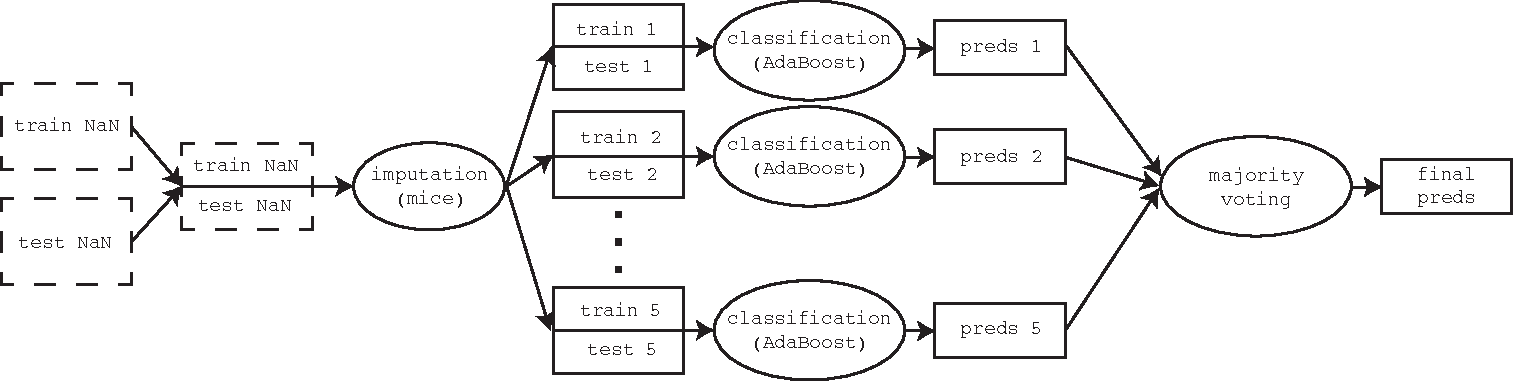
\includegraphics[width=1\columnwidth]{pipeline}
\caption{{\label{fig:pipeline} The figure illustrates the classification pipeline. Matrices are displayed as boxes and methods as ellipses; dashed lines indicate missing values.%
}}
\end{center}
\end{figure}

\section{Results \& Discussion}
\label{sec:results}

In total, I made six submissions during the competition. The best
submission resulted in an accuracy of $85.494\,\%$, which corresponds
to the $3^{\text{rd}}$ position out of $20$ participants at the time
of finishing this report.

In summary, the main challenge lay in handling the missing data
values.  Afterward, standard classification techniques could be
used. The use of different classifiers had no substantial influence on
the achieved accuracy: using a support vector machine, random forest
regression, and AdaBoost classifier resulted in very similar results,
as can be seen in Table~\ref{tab:localpublic}. The use of
semi-supervised methods did not have a substantial effect on the
classification performance; this is in line with findings other
studies, showing that semi-supervised methods do not necessarily lead
to improved performances and can even lead to a lower
accuracy~\cite{zhu2005semi}. It might be that semi-supervised methods
would have had a greater effect, if the number of training samples
would have been substantially smaller.

Since the ground truth labels of the test set were not revealed, error
statistics could only be done based on the 0-1 loss of the public
leaderboard and on the local cross-validation. The restriction of one
submission per day increased the difficulty of the validation. My
public score of $85.494\,\%$---which is only $0.00364$ below the best
performing score in the competition ($85.854\,\%$) and $0.00456$ below
the best performing method of the Delve
project~\footnote{\url{http://www.cs.toronto.edu/~delve/data/adult/adultDetail.html}}---is
an indicator that little improvement will be possible beyond my
system. Compared to the UCI dataset, the given dataset had a smaller
amount of labeled data and more missing values, which made the Kaggle
classification task more challenging. Using standard state-of-the-art
classifiers, the maximum possible performance of the given dataset
will be possibly capped clearly below 100\,\% due to mistakes during
data acquisition, such as deliberate misinformation or transcription
errors. Moreover, the used variables will only have limited
explanatory power: additional variables, such as political view,
morale, or number of children might be needed to increase the amount
of explainable variation.

Due to the concealment of categorical variables, I did not consider
manual feature engineering. Otherwise, it might have been possible to
group certain levels of the categorical (dummy) variables.

Many steps in the classification pipeline were rather time-consuming
and took several hours to complete. In the future, more processing
power could help to increase the classification performance. For
example, using a larger amount of imputed datasets could capture the
uncertainty in the imputed values to a greater degree. The number of
base classifiers---the decision stumps---in the AdaBoost classifier
could be further increased. Moreover, the CPLE framework could be
tested with classifiers that showed good performance in the
cross-validation without transductive learning, such as random forests
or support vector machines.

My code for this competition can be found at:\\
\url{https://github.com/Pold87/ml-final-ass}

\noindent \emph{Word Count}: 2754

\printbibliography


\end{document}

